%% LyX 2.1.4 created this file.  For more info, see http://www.lyx.org/.
%% Do not edit unless you really know what you are doing.
\documentclass[english]{article}
\usepackage[T1]{fontenc}
\usepackage[latin9]{inputenc}
\usepackage{graphicx}

\makeatletter

%%%%%%%%%%%%%%%%%%%%%%%%%%%%%% LyX specific LaTeX commands.
%% Because html converters don't know tabularnewline
\providecommand{\tabularnewline}{\\}

\makeatother

\usepackage{babel}
\begin{document}

\title{Proyect 3: Robotic Finger}


\author{Carlos Alberto Perez Villalta\\
Hector Andres Porras Loria\\
Oscar David Carmona Carvajal}


\date{November 15, 2016}

\maketitle
\newpage{}


\part*{Introduction}

Device drivers are an essential but almost invisible pieces of computing
software that allow us to enjoy the many peripherals we have attached
to our computer. When we attach a computer mouse, usb key or graphic
card, our computer will automatically search and download programs
that will make our devices work perfectly. These programs are known
as device drivers and they basically allow the operating system and
devices to communicate with each other. The purpose of the communication
is to access the hardware resources of the computer by converting
the input/output instructions of the operating system into information
that the device can understand. This occurs because hardware resources
are valuable and thus managed by the operating system, lots of problems
can occur if devices were given direct access to hardware resources
thus that is why the drivers came into existence. In figure 1 we can
see how device drivers basically interact with devices.

\begin{figure}


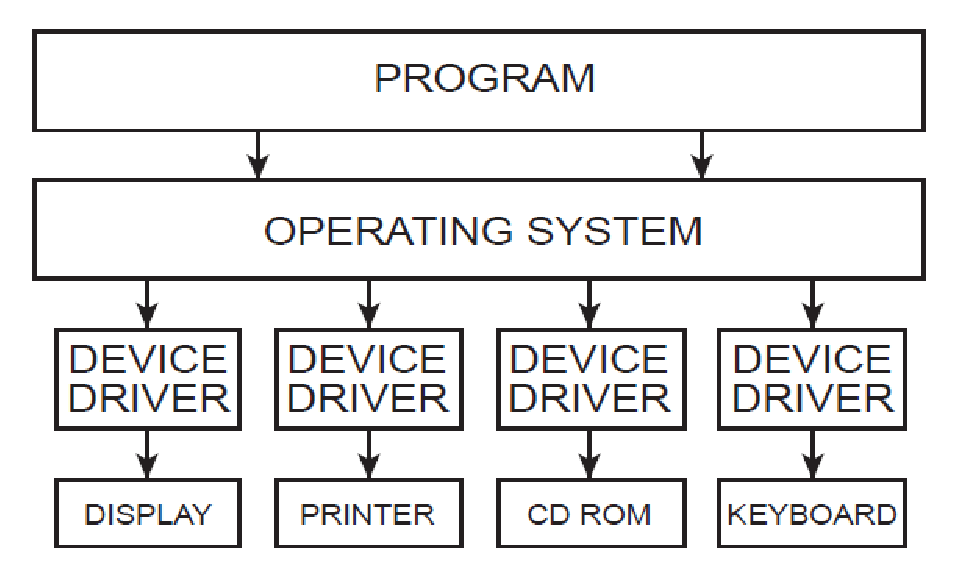
\includegraphics[scale=0.7]{driver}\caption{Device drivers}
\end{figure}


In the Linux operating system drivers are abstracted as files known
as a device special file, the operations we can do in Linux on files
can also be applied to drivers. Each device special file has its own
major and minor device number in order for the operating system to
distinguish the devices. Linux then maps the device special file passed
in system calls to the device's device driver via the major device
number. Once the driver is working, three methods may be used to service
the device:
\begin{itemize}
\item Polling: Basically the operating system waits until the device is
ready to be accessed. Polling is highly recommended for fast devices
that constantly need to be used but it is very wasteful for slow devices
and devices that operate on a much lower frequency. 
\item Interrupts: A method that consists on altering the execution flow
and servicing the device once an external event happens. A basic example
of an interruption is clicking the right button on the mouse. It should
be used on slow devices that depend on an external input.
\item Direct Memory Access: A feature that allows the transfer of data from
the device to memory without having to pass through the central processing
unit. Direct Memory Access or DMA is used for devices that transmit
a very large amount of data and whose performance can be compromised
if it requires to pass through the CPU.
\end{itemize}
Linux provides the kernel memory allocation and deallocation routines
that the devices use to write and read data. Each class of device
driver provides the interface that the kernel uses in order to request
services. {[}1{]}

The third project for the Introduction to Operating Systems course
consists on developing a device driver for a robotic finger that will
input on a keypad. The project is basically divided into two layers:
a software layer and a hardware layer. The hardware level consists
of the robotic finger built on an embedded system thats connected
to a computer. The finger will automatically interact via touching,
pushing and dragging across the screen of a test program built for
mobile devices. The software layer consists of an interpreter that
will read a language created by the programmers that controls the
robot. A device driver built by the programmers will be responsible
for interacting with the physical device, the project will also have
a device library that implements the functions provided by the driver.
Together these two layers compose the third project of this course.


\part*{Development Environment}

The assignment is being developed Ubuntu; a Debian-based Linux operating
system. The programming language being used to develop the project
is C for GNU/Linux (gcc). The Ubuntu version being used for the project
is 16.04. The assignment is being written using the text editor: Visual
Studio Code and gedit. The functions were tested using the inbuilt
debugger tool but mainly via print debugging by compiling the source
files using the linux terminal. Finally for version control we used
Git in order to combine our work and rollback in case of bugs. 

The hardware is being developed on the Arduino micro-controller. The
Arduino allows control over the components that compose the robotic
finger via a series of configurable analog and digital pins. The test
program for Android is being developed using the Ionic framework.
The Ionic framework allows the development of hybrid mobile applications
via the usage of Cordova and AngularJS. The program was first tested
via the built in WebKit browser and later deployed for Android devices.
The interpreter for the custom language was developed in the C language
using Lex and Yacc tools for developing the lexical analyzer and parser. 


\part*{Continuous learning attribute analysis}

In todays information age the environment is constantly changing due
to new developments especially in the field of technology and information.
As Computer Engineers we have to constantly combine our multidisciplinary
knowledge in order to develop innovative solutions to large amount
of problems. The project required a combination of our knowledge in
regards to robotics and electronics with the newly acquired knowledge
of operating systems. 

Mobile and web programming was one of the fields we as computer engineers
applied in the development of a hybrid mobile app. Imperative programming
and memory management was used in the development of the device driver
for a completely costume made robotic finger. The hardware for the
finger required the application of circuit theory and usage of micro
controllers. The combination of all these fields allowed the successful
development of this project. This is not the first nor the last time
we will have to combine our newly acquired information with our learned
skills. 


\part*{Program Design}


\subsection*{Language and Interpreter}

A custom language is necessary in order for the robotic finger to
understand what we want it to do. The following five function were
implement in accordance to the requirements of the project: touch,
push, drag, move and pin. The commands were implemented in the following
language structure:
\begin{itemize}
\item \emph{touch}. This command lowers the finger, touches the screen and
then rises it to the initial position.
\item \emph{push t. }This command lowers the finger, touches the screen
for \emph{t} seconds and then rises to the initial position.
\item \emph{move x y}. This command moves the robotic finger to the position
specified by the \emph{x }horizontal and \emph{y }vertical position. 
\item \emph{drag x y. }This command lowers the finger, touches the screen
and then rises to the initial position. Then it moves to the position
specified by the \emph{x }horizontal and \emph{y }vertical position
and repeats the previous action.
\item \emph{pin n. }This command inputs the pin \emph{n} into the touchscreen.
\end{itemize}
The language was implement using the lex and yacc library. The lex
file defines the structure of the language with the following characteristics:
allowing command to be written in lower and uppercase, ignoring whitespaces
and separating the commands by newline. The yacc file calls the functions
based on the language defined by the lex file, it also checks that
the data is valid such as the range for the \emph{x y }coordinates
for the move and drag command. The functions to be called are all
located on the device driver and the functions will be responsible
for controlling the robotic finger. 


\subsection*{Device Driver and Library}

The device driver is responsible for controlling the arduino device
that controls the robotic hand writing through a USB connection byte
per byte. A character is sent by the USB port and the arduino device
interprets it in order to do a particular action. In Linux all drivers
are treated as files, thus we implemented standard file operations
for the driver file. The following methods were implemented:
\begin{itemize}
\item arduino\_open: Uses the operating system call to open the driver file.
\item arduino\_close: Uses the operating system call to close the driver
file.
\item arduino\_write: Writes a character to the driver file.
\item arduino\_probe: Standard routine to check if everything is working. 
\item arduino\_disconnect: Disconnects the the device. 
\item arduino\_init: Initializes the driver.
\item arduino\_exit: Last thing the driver executes.
\end{itemize}
The read call for the driver was not implemented because it was not
needed and for security reasons it was not implemented. The device
library implements the functions of the robotic finger, the driver
requires the library to understand what to do with the robotic finger.
The following functions were implemented in the library:
\begin{itemize}
\item push: Depending on the state of the finger it sends either the 'p'
or 'P' character. The 'p' character commands the arduino to lowers
the robotic finger while the 'P' character commands the arduino to
lift the finger.
\item touch: Sends the 't' character to command the arduino via the driver
to execute the touch command. The touch command in the driver makes
use of the push to lower and lift the finger.
\item move: The move command sends the position of the desired location
to the arduino via the driver. The move command makes use of the push
command to lower and lift the finger.
\end{itemize}

\subsection*{Test Program}

The usage of the Ionic framework requires the web application to be
developed using web technologies, primarily AngularJS. The tab template
was used to develop the application; each tab containing the different
sized keypads. The keypad, tabs and fields were developed using ionic
CSS components {[}2{]}. The functionality regarding the random pin
generation, pin validation and keyboard input was done using AngularJS
controllers. To guarantee the size of the keys, the ``width'' and
``height'' html attribute were used to define the button size. The
PIN was randomly generated using the random javascript method and
the controller displays a message when the input PIN equals the randomly
generated PIN. The android application for testing the robot with
2cm button size can be seen in Figure 2.

\begin{figure}
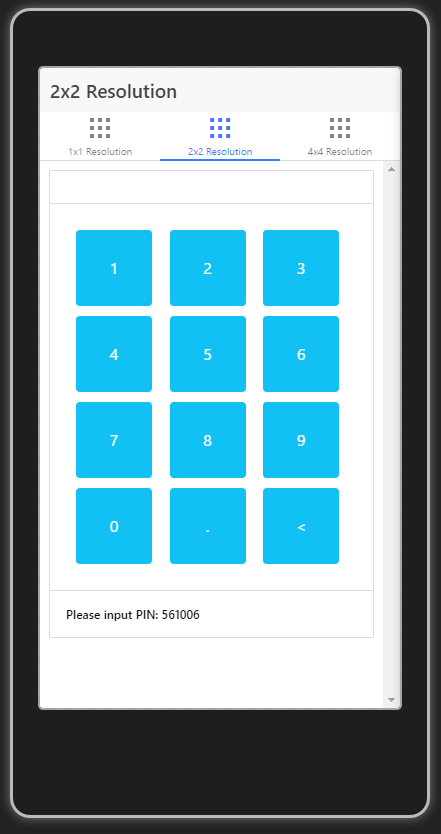
\includegraphics{app}

\caption{Test PIN input Program}
\end{figure}



\subsection*{Robotic Finger}

The hardware for the robotic finger was not developed due to large
time constraints. Instead the team developed a circuit consisting
of light emitting diodes that is compatible with all the robotic finger
driver. Blue LEDs are used to represent the PIN input keypad while
green LEDs are used to represent what the robotic finger is doing. 


\subsection*{UML Diagram}

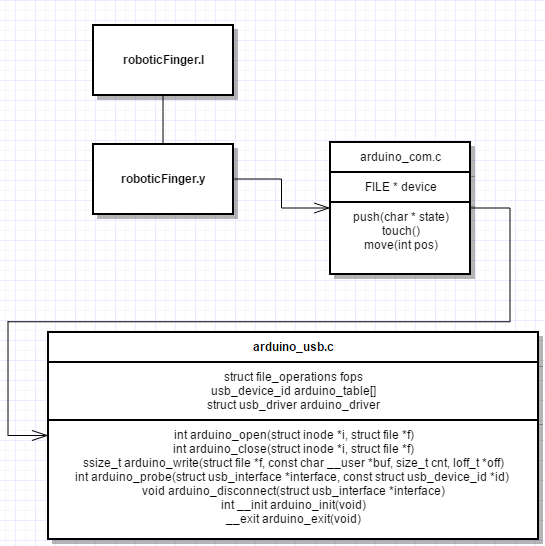
\includegraphics{uml}


\part*{Instructions on how to use program}
\begin{enumerate}
\item Connect the robotic finger to a computer USB port.
\item Navigate to the driver folder.
\item Open a terminal and execute the following commands:

\begin{enumerate}
\item make driver
\item sudo rmmod cdc\_acm
\item sudo insmod arduino\_usb.ko
\item sudo chmod 666 /dev/arduino0
\item sudo chmod 666 /dev/arduino1 
\end{enumerate}
\item Navigate to the lib folder
\item Open a terminal and execute the following commands:

\begin{enumerate}
\item make library
\end{enumerate}
\item Navigate to the src folder and execute the following commands:

\begin{enumerate}
\item make source
\item ./roboticFinger -c conf
\end{enumerate}
\end{enumerate}

\part*{Student activity log}

\begin{tabular}{|c|c|c|c|c|}
\hline 
Assignment & Carlos Perez & Hector Porras & Oscar Carmona & Total Time\tabularnewline
\hline 
\hline 
Language & 0:00 & 1:00 & 0:00 & 1:00\tabularnewline
\hline 
Interpreter & 0:00 & 5:00 & 0:00 & 5:00\tabularnewline
\hline 
Device Driver & 0:00 & 0:00 & 10:00 & 10:00\tabularnewline
\hline 
Device Library & 0:00 & 0:00 & 2:00 & 2:00\tabularnewline
\hline 
Test Application & 5:00 & 0:00 & 0:00 & 5:00\tabularnewline
\hline 
Robotic Finger & 1:00 & 1:00 & 1:00 & 3:00\tabularnewline
\hline 
Documentation & 6:00 & 0:15 & 0:15 & 6:30\tabularnewline
\hline 
Total & 12:00 & 8:15 & 12:15 & 32:30\tabularnewline
\hline 
\end{tabular}


\section*{Project Final Status}

All the sections of project were completed except the hardware. The
hardware was not even attempted due to very serious time constraints
and economic limitations. This was a full group decision and we decided
that it would be better to develop all the other sections. The language,
interpreter, device driver, device library and test application were
all completed successfully. In order to test the functionality of
the driver, we developed a circuit that uses light emitting diodes
in order to demonstrate the project functionality. There were no particular
challenges faced on this project due to the experience the group had
with developing interpreters, mobile applications and drivers. All
group members successfully completed each assigned task on time.


\section*{Conclusion}

Device drivers are one of the most important pieces of software in
existence, they have allowed us to quickly and safely use complicated
devices on our computers. Understanding how drivers work and the methods
they use for getting information is critical in the field of operating
systems. It is suggested that the students attempting to develop similar
projects; have a good background in lexical analysis and parser tools,
mobile application development and C language knowledge. Due to external
time constraints; students attempting to complete this project should
dedicate enough time in the development of the hardware because it
is by far the most time consuming and costliest part of the project.
This project was an excellent experience for the Operating System
course. 
\begin{thebibliography}{1}
\bibitem{key-1}\textquotedblleft Chapter 8 Device Drivers,\textquotedblright{}
The Linux Documentation Project. {[}Online{]}. Available: http://www.tldp.org/ldp/tlk/dd/drivers.html.
{[}Accessed: 12-Nov-2016{]}. 

\bibitem{key-2}D., \textquotedblleft CSS Components,\textquotedblright{}
Ionic. {[}Online{]}. Available: http://ionicframework.com/docs/components/.
{[}Accessed: 13-Nov-2016{]}. \end{thebibliography}

\end{document}
